%-----------------------------------------------------------------------------------------------------------------------------------------------%
%	The MIT License (MIT)
%
%	Copyright (c) 2022 Dinis Anatoliy
%
%	Permission is hereby granted, free of charge, to any person obtaining a copy
%	of this software and associated documentation files (the "Software"), to deal
%	in the Software without restriction, including without limitation the rights
%	to use, copy, modify, merge, publish, distribute, sublicense, and/or sell
%	copies of the Software, and to permit persons to whom the Software is
%	furnished to do so, subject to the following conditions:
%	
%	THE SOFTWARE IS PROVIDED "AS IS", WITHOUT WARRANTY OF ANY KIND, EXPRESS OR
%	IMPLIED, INCLUDING BUT NOT LIMITED TO THE WARRANTIES OF MERCHANTABILITY,
%	FITNESS FOR A PARTICULAR PURPOSE AND NONINFRINGEMENT. IN NO EVENT SHALL THE
%	AUTHORS OR COPYRIGHT HOLDERS BE LIABLE FOR ANY CLAIM, DAMAGES OR OTHER
%	LIABILITY, WHETHER IN AN ACTION OF CONTRACT, TORT OR OTHERWISE, ARISING FROM,
%	OUT OF OR IN CONNECTION WITH THE SOFTWARE OR THE USE OR OTHER DEALINGS IN
%	THE SOFTWARE.
%	
%
%-----------------------------------------------------------------------------------------------------------------------------------------------%


%============================================================================%
%
%	DOCUMENT DEFINITION
%
%============================================================================%

%we use article class because we want to fully customize the page and don't use a cv template
\documentclass[10pt,A4]{article}	


%----------------------------------------------------------------------------------------
%	ENCODING
%----------------------------------------------------------------------------------------

%we use utf8 since we want to build from any machine
\usepackage[utf8]{inputenc}		

%----------------------------------------------------------------------------------------
%	LINKS	
%----------------------------------------------------------------------------------------

%Create clickable links from urls
\usepackage[hidelinks]{hyperref}

%----------------------------------------------------------------------------------------
%	LOGIC
%----------------------------------------------------------------------------------------

% provides \isempty test
\usepackage{xifthen}

%----------------------------------------------------------------------------------------
%	FONT
%----------------------------------------------------------------------------------------

% some tex-live fonts - choose your own

%\usepackage[defaultsans]{droidsans}
%\usepackage[default]{comfortaa}
%\usepackage{cmbright}
%\usepackage[default]{raleway}
%\usepackage{fetamont}
%\usepackage[default]{gillius}
%\usepackage[light,math]{iwona}
\usepackage[thin]{roboto} 

% set font default
\renewcommand*\familydefault{\sfdefault} 	
\usepackage[T1]{fontenc}

% more font size definitions
\usepackage{moresize}		


%----------------------------------------------------------------------------------------
%	PAGE LAYOUT  DEFINITIONS
%----------------------------------------------------------------------------------------

%debug page outer frames
%\usepackage{showframe}			


%define page styles using geometry
\usepackage[a4paper]{geometry}		

% for example, change the margins to 2 inches all round
\geometry{top=1.75cm, bottom=-.6cm, left=1.5cm, right=1.5cm} 	

%use customized header
\usepackage{fancyhdr}				
\pagestyle{fancy}

%less space between header and content
\setlength{\headheight}{-5pt}		


%customize entries left, center and right
\lhead{}
\chead{ \small{Dinis Anatoliy  $\cdot$ Applications Engineer $\cdot$  Tokyo, Japan $\cdot$  \textcolor{sectcol}{\textbf{anatoliy.dinis@gmail.com}}  $\cdot$ +81 070 8489 2958 }}
\rhead{}


%indentation is zero
\setlength{\parindent}{0mm}

%----------------------------------------------------------------------------------------
%	TABLE /ARRAY DEFINITIONS
%---------------------------------------------------------------------------------------- 

%for layout-ing tables
\usepackage{multicol}			
\usepackage{multirow}

%extended aligning of tabular cells
\usepackage{array}

\newcolumntype{x}[1]{%
>{\raggedleft\hspace{0pt}}p{#1}}%


%----------------------------------------------------------------------------------------
%	GRAPHICS DEFINITIONS
%---------------------------------------------------------------------------------------- 

%for header image
\usepackage{graphicx}

%for floating figures
\usepackage{wrapfig}
\usepackage{float}
%\floatstyle{boxed} 
%\restylefloat{figure}

%for drawing graphics		
\usepackage{tikz}				
\usetikzlibrary{shapes, backgrounds,mindmap, trees}


%----------------------------------------------------------------------------------------
%	Color DEFINITIONS
%---------------------------------------------------------------------------------------- 

\usepackage{color}

%accent color
\definecolor{sectcol}{RGB}{255,150,0}

%dark background color
\definecolor{bgcol}{RGB}{10,10,10}

%light background / accent color
\definecolor{softcol}{RGB}{225,225,225}


%============================================================================%
%
%
%	DEFINITIONS
%
%
%============================================================================%

%----------------------------------------------------------------------------------------
% 	HEADER
%----------------------------------------------------------------------------------------

% remove top header line
\renewcommand{\headrulewidth}{0pt} 

%remove bottom header line
\renewcommand{\footrulewidth}{0pt}	  	

%remove page-num
\renewcommand{\thepage}{}	

%remove section num		
\renewcommand{\thesection}{}			

%----------------------------------------------------------------------------------------
% 	ARROW GRAPHICS in Tikz
%----------------------------------------------------------------------------------------

% a six pointed arrow pointing to the left
\newcommand{\tzlarrow}{(0,0) -- (0.2,0) -- (0.3,0.2) -- (0.2,0.4) -- (0,0.4) -- (0.1,0.2) -- cycle;}	

% include the left arrow into a tikz picture
% param1: fill color
%
\newcommand{\larrow}[1]
{\begin{tikzpicture}[scale=0.58]
	 \filldraw[fill=#1!100,draw=#1!100!black]  \tzlarrow
 \end{tikzpicture}
}

% a six pointed arrow pointing to the right
\newcommand{\tzrarrow}{ (0,0.2) -- (0.1,0) -- (0.3,0) -- (0.2,0.2) -- (0.3,0.4) -- (0.1,0.4) -- cycle;}

% include the right arrow into a tikz picture
% param1: fill color
%
\newcommand{\rarrow}
{
\begin{tikzpicture}[scale=0.7]
	\filldraw[fill=sectcol!100,draw=sectcol!100!black] \tzrarrow
 \end{tikzpicture}
}



%----------------------------------------------------------------------------------------
%	custom sections
%----------------------------------------------------------------------------------------

% create a coloured box with arrow and title as cv section headline
% param 1: section title
%
\newcommand{\cvsection}[1]
{
\colorbox{sectcol}{\mystrut \makebox[1\linewidth][l]{
\larrow{bgcol} \hspace{-7pt} \larrow{bgcol} \hspace{-7pt} \larrow{bgcol} \textcolor{white}{\textbf{#1}}\hspace{4pt}
}}\\
}

%create a coloured arrow with title as cv meta section section
% param 1: meta section title
%
\newcommand{\metasection}[2]
{
\begin{tabular*}{1\textwidth}{p{2.4cm} p{11cm}}
\larrow{bgcol}	\normalsize{\textcolor{sectcol}{#1}}&#2\\[12pt]
\end{tabular*}
}

%----------------------------------------------------------------------------------------
%	 CV EVENT
%----------------------------------------------------------------------------------------

% creates a stretched box as cv entry headline followed by two paragraphs about 
% the work you did
% param 1:	event time i.e. 2014 or 2011-2014 etc.
% param 2:	event name (what did you do?)
% param 3:	institution (where did you work / study)
% param 4:	what was your position
% param 5:	some words about your contributions
%
\newcommand{\cvevent}[5]
{
\vspace{8pt}
	\begin{tabular*}{1\textwidth}{p{3cm}  p{10.8cm} x{3.9cm}}
 \textcolor{bgcol}{#1}& \textbf{#2} & \vspace{2.5pt}\textcolor{sectcol}{#3}

	\end{tabular*}
\vspace{-12pt}
\textcolor{softcol}{\hrule}
\vspace{6pt}
	\begin{tabular*}{1\textwidth}{p{3cm} p{14.4cm}}
&		 \larrow{bgcol}  #4\\[3pt]
\ifx#5\empty
\else
&		 \larrow{bgcol}  #5\\[6pt]
\fi
	\end{tabular*}

}

% creates a stretched box as 
\newcommand{\cveventmeta}[2]
{
	\mbox{\mystrut \hspace{87pt}\textit{#1}}\\
	#2
}

%----------------------------------------------------------------------------------------
% CUSTOM STRUT FOR EMPTY BOXES
%----------------------------------------- -----------------------------------------------
\newcommand{\mystrut}{\rule[-.3\baselineskip]{0pt}{\baselineskip}}

%============================================================================%
%
%
%
%	DOCUMENT CONTENT
%
%
%
%============================================================================%
\begin{document}


%use our custom fancy header definitions
\pagestyle{fancy}	


%---------------------------------------------------------------------------------------
%	TITLE HEADLINE
%----------------------------------------------------------------------------------------
\vspace{-20.55pt}

% use this for multiple words like working titles etc.
%\hspace{-0.25\linewidth}\colorbox{bgcol}{\makebox[1.5\linewidth][c]{\hspace{46pt}\HUGE{\textcolor{white}{\textsc{Dinis Anatoliy}} } \textcolor{sectcol}{\rule[-1mm]{1mm}{0.9cm}} \parbox[b]{5cm}{   \large{ \textcolor{white}{{IT Consultant}}}\\
% \large{ \textcolor{white}{{Resume}}}}
%}}

% use this for single words, e.g. CV or RESUME etc.
\hspace{-0.25\linewidth}\colorbox{bgcol}{\makebox[1.5\linewidth][c]{\HUGE{\textcolor{white}{\textsc{Dinis Anatoliy}} } \textcolor{sectcol}{\rule[-1mm]{1mm}{0.9cm}} \HUGE{\textcolor{white}{\textsc{Resume}} } }}


%----------------------------------------------------------------------------------------
%	HEADER IMAGE
%----------------------------------------------------------------------------------------

\begin{figure}[H]
\begin{flushright}
	%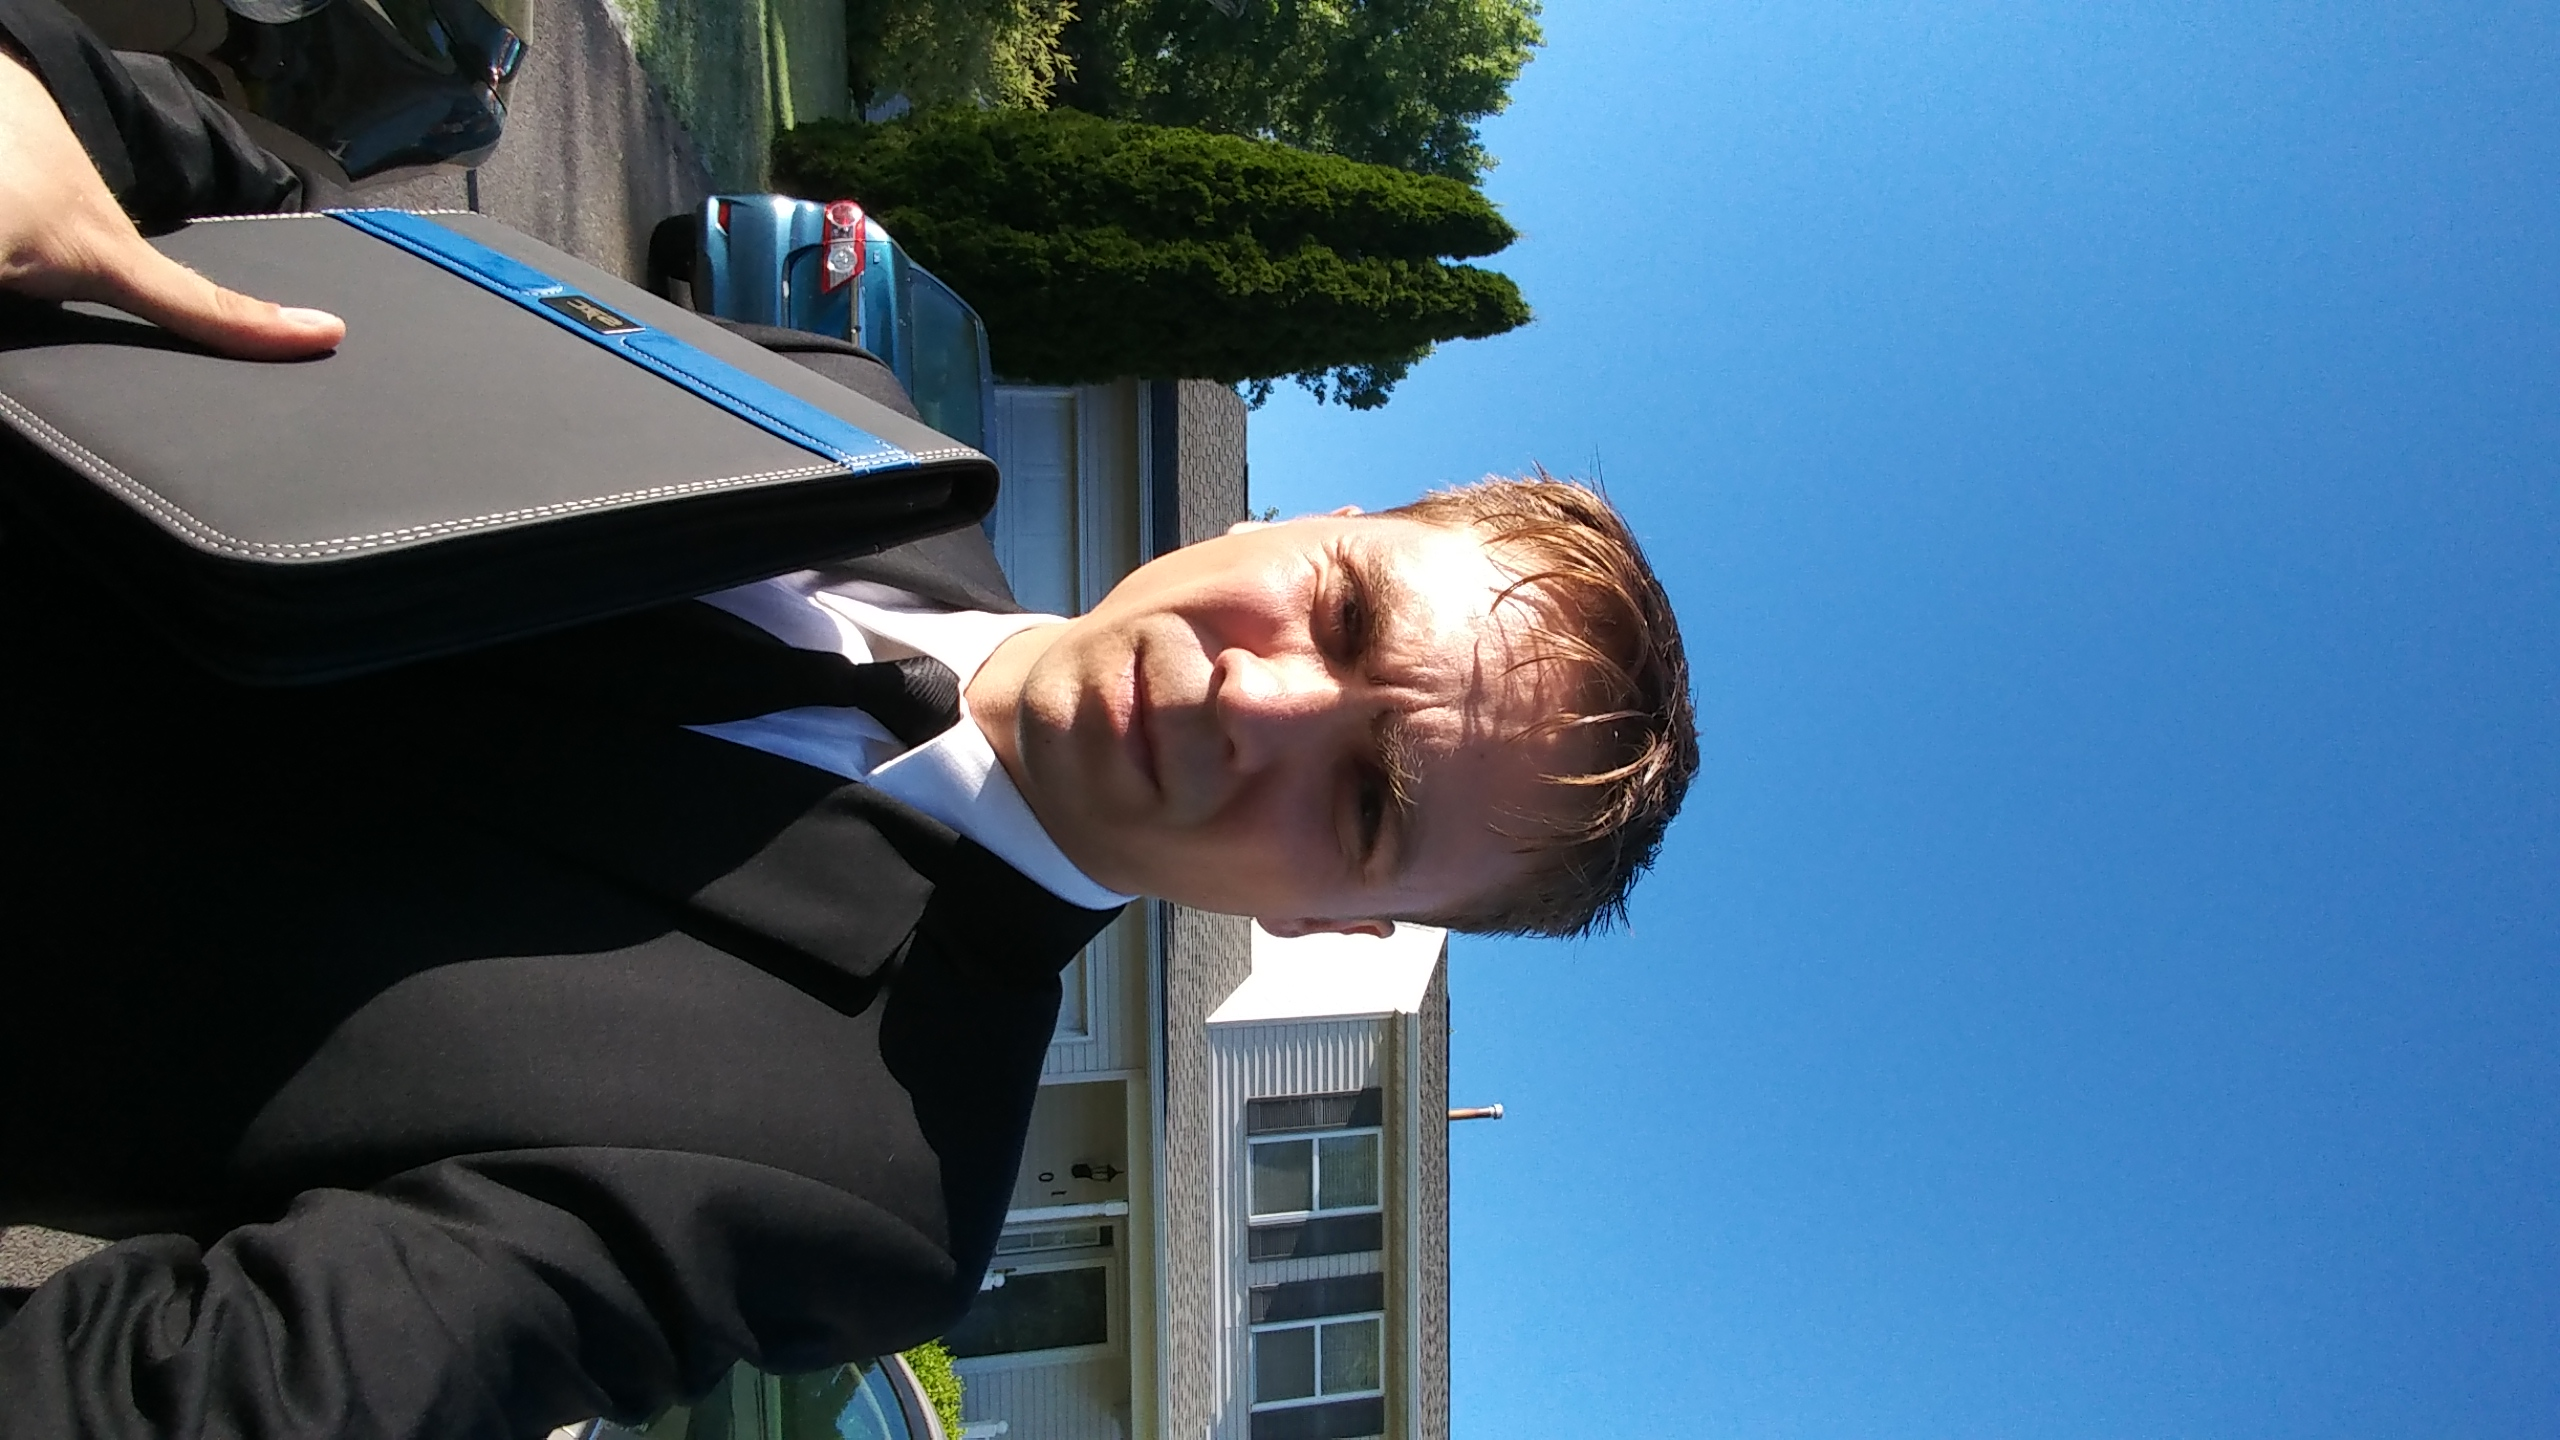
\includegraphics[trim= 320 130 460 210,clip,width=0.2\linewidth]{myphoto.jpg}	%trimming relative to image size!
	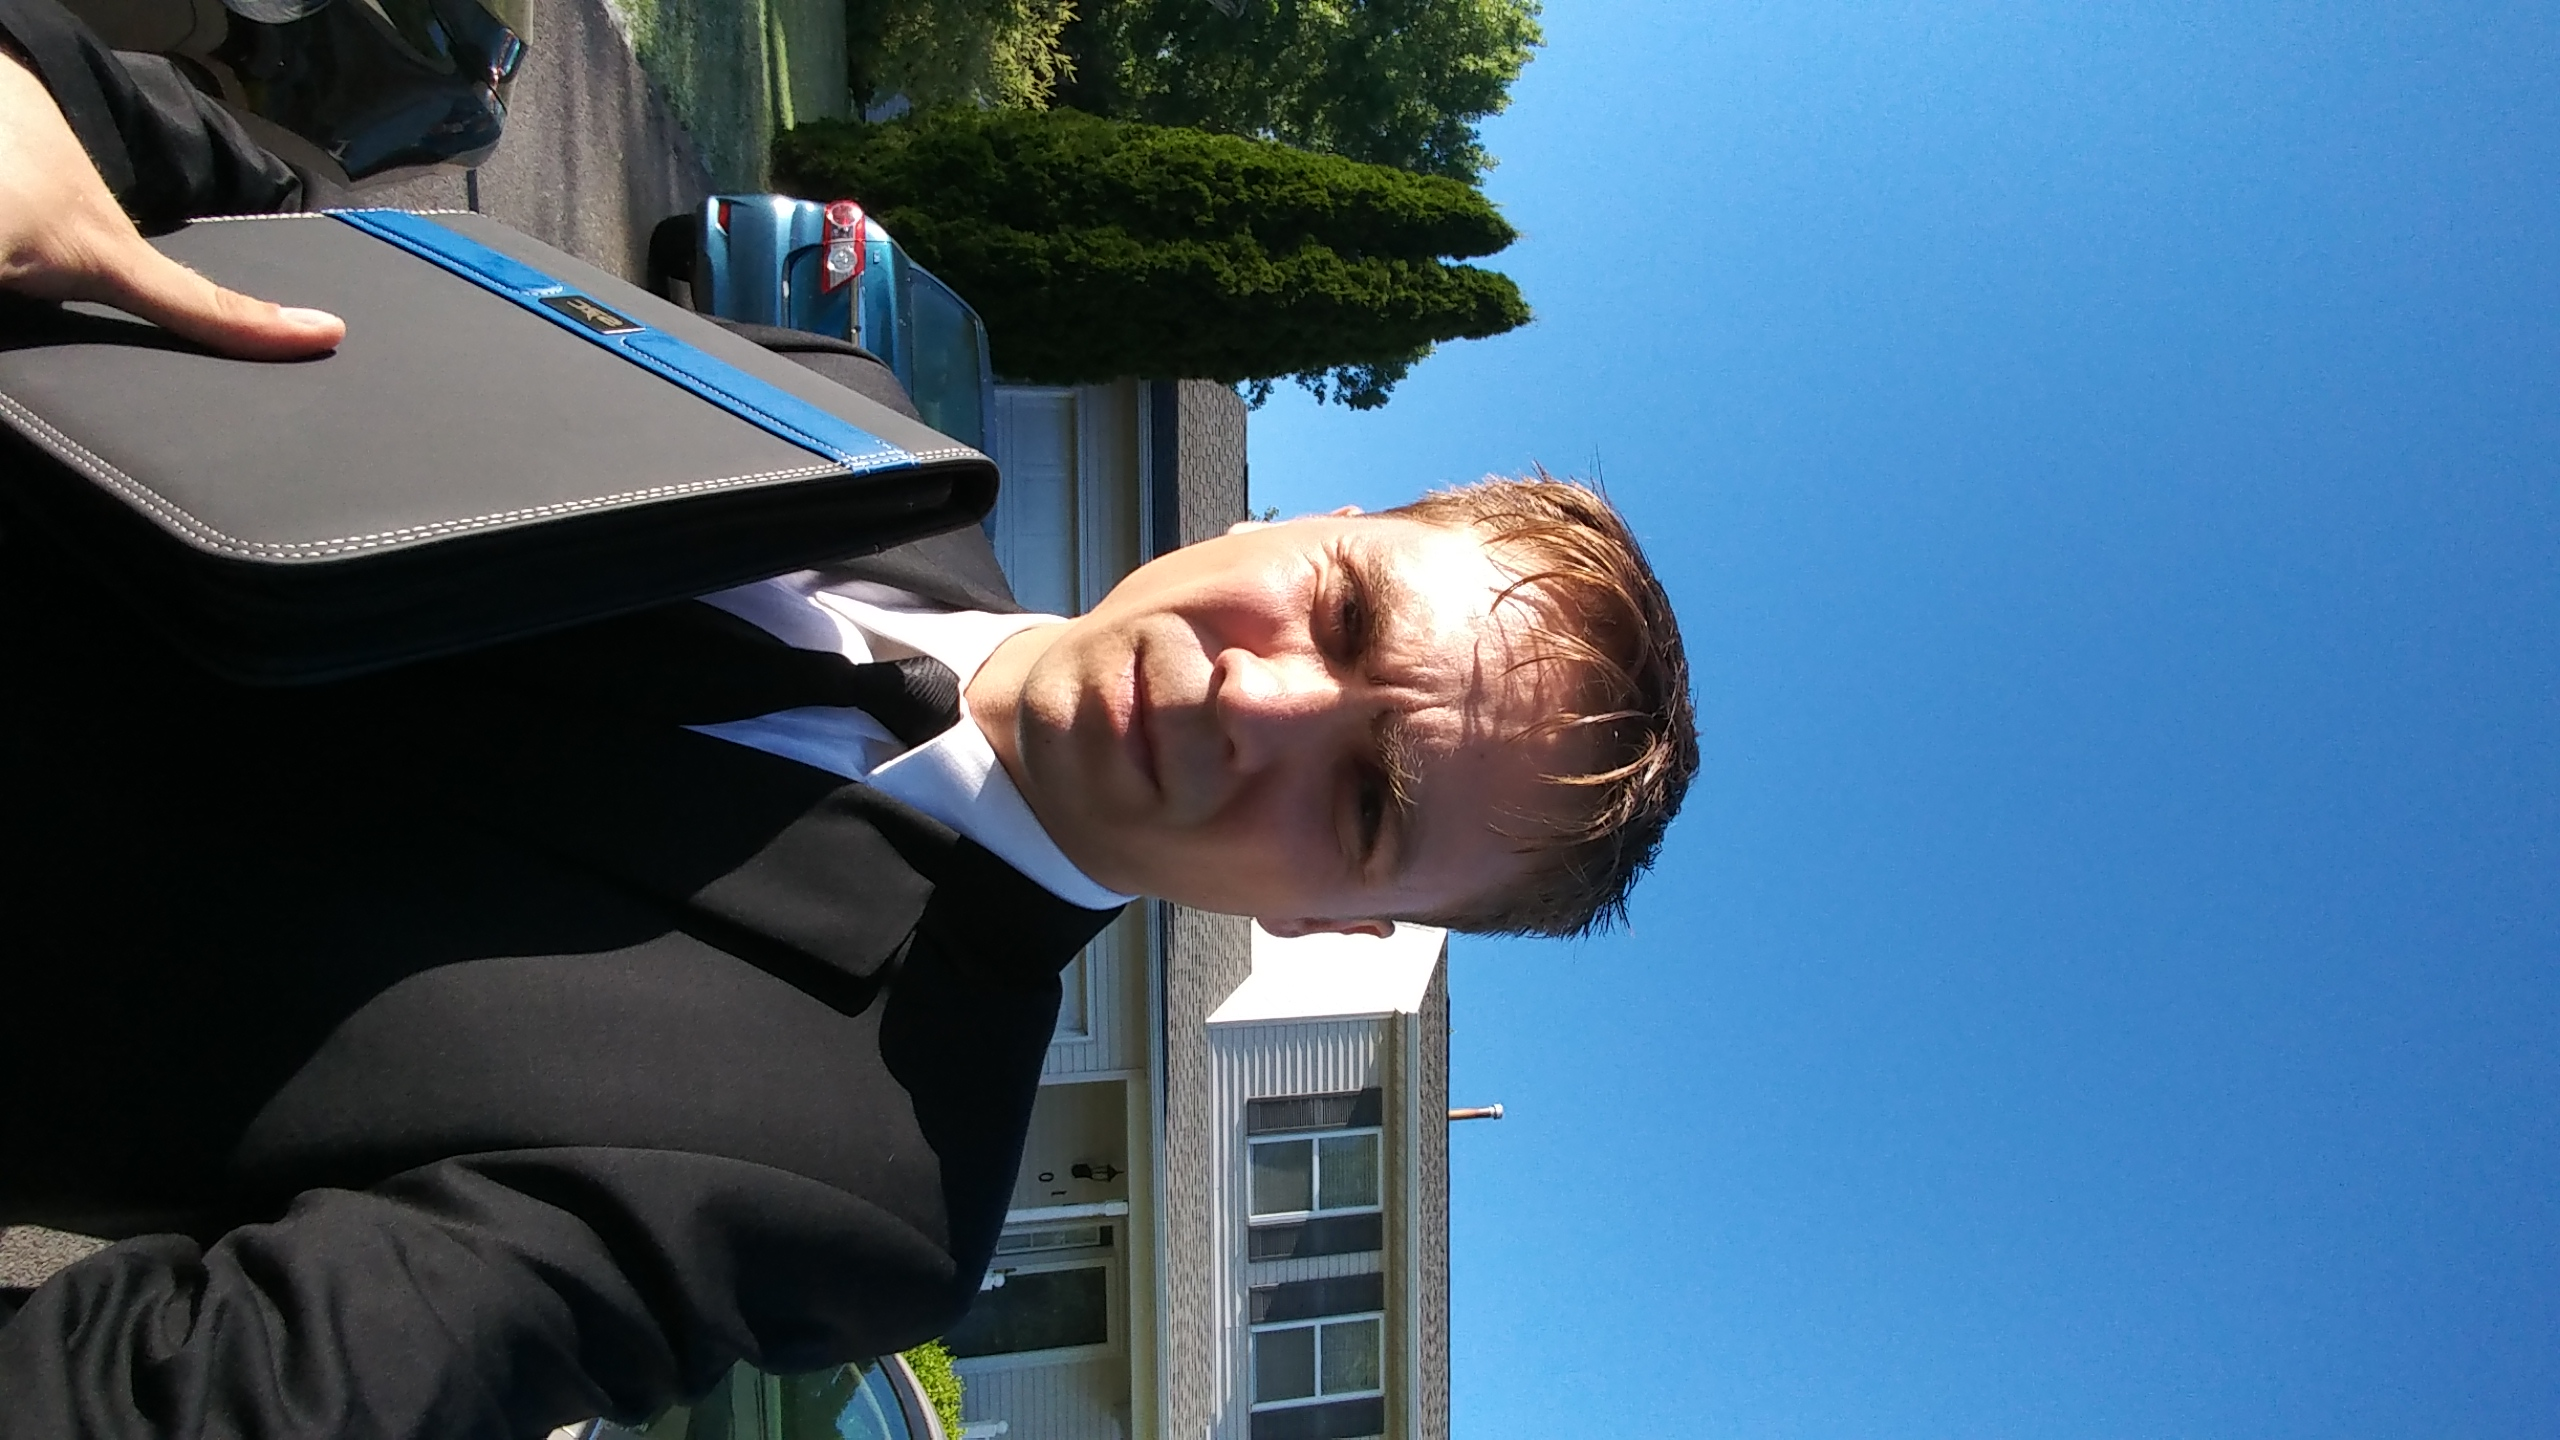
\includegraphics[angle=90,trim= 800 250 800 250,clip,width=0.2\linewidth]{myphoto.jpg}	%trimming relative to image size!
\end{flushright}
\end{figure}

%---------------------------------------------------------------------------------------
%	QR CODE (optional)
%----------------------------------------------------------------------------------------
%\vspace{-136pt}
%\hspace{0.75\linewidth}
%\includegraphics[width=103pt]{qrcode}
%\normalsize
%\vspace{88pt}

%---------------------------------------------------------------------------------------
%	META SECTION
%----------------------------------------------------------------------------------------

\vspace{-114pt}

\metasection{Status:}{B.Sc. Computer Science, Applications Engineer}
\metasection{Fields:}{Project Management, Software Development, Research} 
\metasection{Tech:}{Ruby on Rails, Redis, Jenkins,  Kubernetes, Linux, Kotlin, Java, C\#, C++, Python }
\metasection{Loves:}{RPGs, Art, Comedy Series, Soccer, Fitness}

\vspace{6pt}

%---------------------------------------------------------------------------------------
%	SUMMARY (optional)
%----------------------------------------------------------------------------------------

\cvsection{Summary}\\
I am a Computer Science graduate (B.Sc.) with project experience working on large scale Air Traffic Surveillance Software written mostly in C/C++; with some services and scripts in Java, Bash and Python, running on linux racks during University as well as after. I moved to Japan in 2019 and worked at multiple Japanese companies where I learned to develop for IoT devices, prepare and release phase 2 requirements and features for an automated email distribution system running on K8S, enhance a game engine solution that extends Unity and Unreal Engine with Kotlin and create solution to deploy/test micro-services to K8S with CI/CD.\\

Currently I am working on a Ruby on Rails application to upgrade to currently supported versions, fix integration tests and automatically deploy to K8S with a CI/CD pipeline as well as an outsourced Java application that needs to be understood, refactored, fixed and documented.\\[-2pt]

%============================================================================%
%
%	CV SECTIONS AND EVENTS (MAIN CONTENT)
%
%============================================================================%

%---------------------------------------------------------------------------------------
%	EXPERIENCE
%----------------------------------------------------------------------------------------
\cvsection{Experience}

%
\cvevent{2022 / 09}{Applications Engineer}{Rakuten, Inc.}{Working on Ruby on Rails application that needs to Rails and Ruby versions upgraded and automatic deployment/testing on Ci/CD pipeline}{Learning and documenting outsourced Java application and fixing/refactoring logic.}

%\textcolor{softcol}{\hrule}

%
\cvevent{2022 / 01 - 2022 / 07}{Research and Development Engineer}{Softgear Co., Ltd.}{Strix Game Engine Research and Development}{Implement new features for micro services for Strix Game Engine with Unity and Unreal Engine as well as work on testing and adding features for outsourced Games created with Strix Engine}

%\textcolor{softcol}{\hrule}

%
\cvevent{2020 / 06 - 2021 / 12}{Software Engineer}{Rakuten, Inc.}{Phase 2 Features and Refactoring of Automatic Email Distribution System}{Implemented new features with unit, integration and end-to-end tests, deployed to automatic CI/CD and help release on Production}


%\textcolor{softcol}{\hrule}

%
\cvevent{2019 / 07 - 2020 / 05}{Embedded Software Engineer}{Jigsaw, Inc.}{Managed team to develop libraries for different sensors that connect to Neqto IoT device to collect sensor data and send to cloud}{Converted libraries from Python/C/C++ to Javascript and added features to allow sending data to different cloud platforms like AWS S3, IoT Core, Dropbox, Azure, Salesforce, etc.}

%\textcolor{softcol}{\hrule}

%
\cvevent{2018 / 06 - 2019 / 06}{Software Engineer}{SRC, Inc.}{Worked on proprietary simulation software for air trafic control}{Created application to parse large json simulation files and create formatted word document of data as well as maintained and fixed bugs for radar systems integrated with VHDL}

%\textcolor{softcol}{\hrule}

%
\cvevent{2016 / 02 - 2018 / 12}{Software Engineer Co-Op}{Saab Sensis Corporation}{Worked on porting large air traffic services from running on bare metal to KVM}{Built custom rpm packages to automate prepartion of bare metal systems. Project leader in creating Java GUI application set ASTERIX settings. Maintained SNMP agent to monitor MIBs. Restructured, tested and maintained Ruby cookbooks to configure VNC environments and networks on VMs. Maintained and fixed multiliterate time synchronization issues of application to run simulations of air traffic and surveillance hardware.}


%---------------------------------------------------------------------------------------
%	EDUCATION SECTION
%--------------------------------------------------------------------------------------
\cvsection{Education}

\cvevent{2018 / 05}{Graduated}{Syracuse University}{After returning from Study Abroad}{Graduated with a 3.4 GPA and started working at SRC, Inc. in June 2018.}

%\textcolor{softcol}{\hrule}

%
\cvevent{2018 / 01 - 2018 / 05}{Semester Abroad in Osaka, Japan}{Kansai Gaidai University}{Studied Japanese, Culture, Religion}{Took a semester in Japan because I've always wanted to go to Japan and have been taking Japanese language courses as an elective.}

%\textcolor{softcol}{\hrule}

%
\cvevent{2015 - 2017}{B.Sc. Computer Science}{Syracuse University}{Dean's Scholarship}{Main languages that were taught at Syracuse were Haskell, Java and C. Studied networking and Android programming. Took Japanese as an elective for 3 semesters.}

%\textcolor{softcol}{\hrule}

%
\cvevent{2014 - 2015}{A.Sc. Computer Science}{Onondaga Community College}{Curriculum Honor Award Computer Science, 2016}{Began learning programming with mostly Java and C++. Took a web development class focused on html and css. Graduated with a 3.7 GPA.}

%---------------------------------------------------------------------------------------
%	LANGUAGE SECTION
%--------------------------------------------------------------------------------------
\cvsection{Language}

%
\cvevent{English}{Fluent}{United States of America}{Moved to USA in 1990}{Grew up in Upstate New York and went to school in Syracuse from Kindergarten to University}

%\textcolor{softcol}{\hrule}

%
\cvevent{Japanese}{Intermediate}{University}{Studied Abroad at Kansai Gaidai in 2018 for 1 Semester}{Took 3 semesters of Japanese language classes and am continueing self study}

%\textcolor{softcol}{\hrule}

%
\cvevent{Ukrainian}{Basic}{Home}{Born in Ukraine in 1987}{Moved to USA at the age of 4 and learned some Ukrainian from home life as well as family members, friends and church.}

%---------------------------------------------------------------------------------------
%	CONTACT SECTION
%--------------------------------------------------------------------------------------
\cvsection{Contact}

%
\cvevent{GitHub}{\href{https://github.com/ad2phnx}{github.com/ad2phnx}}{}{Personal Code Repository}{Projects include linux configurations, code test projects for different positions, personal projects, resume.}

%\textcolor{softcol}{\hrule}

%
\cvevent{LinkedIn}{\href{https://www.linkedin.com/in/anatoliy-dinis/}{linkedin.com/in/anatoliy-dinis}}{}{Work and Education History Profile}{}

%\textcolor{softcol}{\hrule}

%
\cvevent{CodeWars}{\href{https://www.codewars.com/users/ad2phnx}{codewars.com/users/ad2phnx}}{}{Coding Challenges Website}{Member since 2015 with a rank of 3Kyu and honor percentile of 1.34\%Completed over 350 challenges in a a variety of different coding languages such as Ruby, Python, Java, SQL, PHP, Go, etc.}

%-------------------------------------------------------------------------------------------------
%	ARTIFICIAL FOOTER (fancy footer cannot exceed line width) 
%--------------------------------------------------------------------------------------------------

\null
\vspace*{\fill}
\hspace{-0.25\linewidth}\colorbox{bgcol}{\makebox[1.5\linewidth][c]{\mystrut \small \textcolor{white}{adtwo.net} $\cdot$ \textcolor{white}{github.com/ad2phnx}}}




%============================================================================%
%
%
%
%	DOCUMENT END
%
%
%
%============================================================================%
\end{document}
